%% ****** Start of file authguide.tex ****** %
%%
%%   This file is part of the APS files in the REVTeX 4 distribution.
%%   Version 4.1r of REVTeX, August 2010
%%
%%   Copyright (c) 2009, 2010 The American Physical Society.
%%
%%   See the REVTeX 4.1 README file for restrictions and more information.
%%
\listfiles
\documentclass[%
,aps%
 ,twocolumn%
 ,secnumarabic%
,amssymb, amsmath,nobibnotes, aps, prl, floatfix]{revtex4-1}
\usepackage{docs}%
\usepackage{bm}%
%\usepackage[colorlinks=true,linkcolor=blue]{hyperref}%
%\nofiles
\expandafter\ifx\csname package@font\endcsname\relax\else
 \expandafter\expandafter
 \expandafter\usepackage
 \expandafter\expandafter
 \expandafter{\csname package@font\endcsname}%
\fi

\begin{document}

\title{\revtex~4.1 Author's Guide}%
\author{American Physical Society}%
\email{revtex@aps.org}
\affiliation{1 Research Road, Ridge, NY 11961}
\date{August 2010}%
\maketitle
\tableofcontents
\clearpage
\section{Introduction}

This is the author's guide to \revtex~4.1, the preferred submission
format for all APS and AIP journals. This guide is intended to be a concise
introduction to \revtex~4.1. The documentation has been separated out
into smaller units to make it easier to locate essential
information.

The following documentation is also part of the \revtex~4.1
distribution. Updated versions of these will be maintained at
the \revtex~4.1 homepage located at \url{http://authors.aps.org/revtex4/}.
\begin{itemize}
\item \textit{APS Author Guide for \revtex~4.1}
\item \textit{Author's Guide to AIP Substyles for \revtex~4.1}
\item \textit{\revtex~4.1 Command and Options Summary}
\item \textit{What's New in  \revtex~4.1}
\end{itemize}
This guide assumes a working \revtex~4.1
installation. Please see the installation instructions included with the
distribution.
\subsection{Changes in \revtex~4.1}
The \revtex\ system for \LaTeX\ began its development in 1986 and has
gone through three major revisions since then.  \revtex~4 was released in August, 2001. Since that time,
many user requests for new features were received. The main goals for  \revtex~4.1 are to incorporate
this user feedback and provide support for the journals of the American Institute of Physics (AIP) . It incorporates the following changes:

\begin{itemize}
\item \textbf{Added support for APS journal \textit{Physical Review Special Topics -- Physics Education Research}}.
\item \textbf{Added support for AIP journals.} There is now an explicit \texttt{aip} society option along with support for AIP journals. Please see the \textit{Author's Guide to AIP Substyles for \revtex~4.1}. In addition, \revtex~4.1 provides an extensible system for the easy addition of new collections of journals.
\item \textbf{Endnotes now ordered correctly.} Endnotes in the bibliography now appear in the correct order, interleaved with citations.
\item \textbf{Multiple references in a single citation supported using a special starred (*) argument to the \cmd\cite\ command.} One of the major new features in 4.1 made possible by the joint work on \texttt{natbib 8.3}. Multiple Bib\TeX\ entries can be combined into a single \cmd\bibitem\ command.
\item \textbf{Free form text can be prepended and appended to a bibliographic entry using the special starred (*) argument to the \cmd\cite\ command.} Often a citation in the bibliography will have explanatory text such as \textit{See also} or \textit{and references therein} before and after the actual citation. The new \revtex~4.1 \cmd\cite\ command allows the specification of both text to precede and follow a citation.
\item \textbf{Structured Abstracts.} Use of the \texttt{description} environment in abstracts now provides for ``structured" abstracts.
\item \textbf{Figures referring to videos now supported.} A ``figure" may now be labeled as a \textbf{Video} by using the \texttt{video} environment. A frame from the video may be included in the figure and a URL to link the caption's label to the online video also may be included. There is also a \cmd\listofvideos\ command.
\item \textbf{Better support for arXiv.org in Bib\TeX\ } Three more Bib\TeX\ fields have been added: \texttt{SLACcitation}, \texttt{archivePrefix}, and \texttt{primaryClass} in addition to the existing field \texttt{eprint}. 
\item \textbf{Improved Bib\TeX\ \texttt{bst} files.} In addition to the new features above, numerous other improvements to the APS \texttt{bst} files have been made, including support for displaying journal article titles (using the new \texttt{longbibliography} option) and many fixes for \textit{Reviews of Modern Physics}. Also, long author lists are no longer automatically truncated.
\item \textbf{\cmd\footnote\ in \cmd\widetext\ and \texttt{table*} environments improved.} \cmd\footnote\relax s in  the \cmd\widetext\ or \texttt{table*} environments are now correctly placed and formatted.
\item \textbf{Email addresses no longer print twice on papers less than one page long.}
\item \textbf{\texttt{eqnarray} alignment improved.}
\item \textbf{\cmd\collaboration\ can be used with the \texttt{groupedaddress} option now.}
\item \textbf{\texttt{letterpaper} now ensured as default paper size.} 
\item \textbf{Table of Contents formatting improved.}
\item \textbf{Support for the \texttt{longtable} package improved.}
\item \textbf{\texttt{reftest} restored.}
\item \textbf{Compatibility with the \texttt{geometry, lineno, lscape} and \texttt{colortbl} packages improved.} For line numbering, rather than using \texttt{lineno.sty} directly, the \texttt{linenumbers} class option should be used (this will call in \texttt{lineno.sty} with a proper set of default parameters).
\item \texttt{hyperref} \textbf{fixes}. Improvements were to make footnotes work better with the \texttt{hyperref} package. In particular, table footnotes were fixed. More anchors for \texttt{hyperref} were also added (titlepage, abstract, and acknowledgements).
\item \textbf{Documents can have more than 256 \cmd\cite\ commands now.}
\item \textbf{\cmd\listoffigures\ and \cmd\listoftables\ fixed.}
\item \textbf{Figure and table labels in captions now reflect proper APS style.}
\item \textbf{RMP style files conform better to RMP style guidelines.}
\item \textbf{Section heading upper-casing improved.}
\item \textbf{Repeated characters at start of affiliation no longer disappear when using \texttt{groupedaddress} option.}
\item \textbf{There have been many other bug fixes and improvements to the internal \texttt{ltxgrid} package as well.}
\end{itemize}

\subsection{\revtex~4 Backwards Compatibility}
Documents prepared under \revtex~4 should process correctly under \revtex~4.1. However, the formatting of the pages and, if using Bib\TeX, the references may change.



\subsection{Submitting to APS Journals}

Authors using \revtex~4.1 to prepare a manuscript for submission to
\textit{Physical Review Letters}, \textit{Physical Review},  \textit{Reviews of Modern Physics}, 
or other APS journals must also read the companion document \textit{APS Author Guide for \revtex~4.1}
distributed with \revtex\ and follow the guidelines detailed there.

The \revtex~4.1 distribution includes both a template
(\file{apstemplate.tex}) and a sample document (\file{apssamp.tex}).
The template is a good starting point for a manuscript. In the
following sections are instructions that should be sufficient for
creating a paper using \revtex~4.1.

Further information about submissions to the American
Physical Society may be found at \url{http://publish.aps.org/}.

\subsection{Submitting to AIP Journals}

\revtex~4.1 includes support for the journals of the American Institute of Physics.
The style files and authoring guides for these journals are distributed as part
\revtex~4.1 distribution. The distribution includes both a template
(\file{aiptemplate.tex}) and a sample document (\file{aipsamp.tex}).
The template is a good starting point for a manuscript. In the
following sections are instructions that should be sufficient for
creating a paper using \revtex~4.1.



More information may be found at 
\url{http://www.aip.org/pubservs/compuscript.html}. Please consult the \textit{Author's Guide to AIP Substyles for \revtex~4.1} for more information about submissions to AIP journals, AIP styles files, and other AIP-specific information.

\subsection{Contact Information}\label{sec:aipresources}%
Any bugs, problems, or inconsistencies with \revtex\ or the APS journal style files should be reported to
\revtex\ support at \verb+revtex@aps.org+. Reports should include information on the error and a \textit{small}
sample document that manifests the problem if possible (please don't send large files!). Issues related to the AIP journal styles should be sent directly to \verb+tex@aip.org+.

\section{Some \LaTeXe\ Basics}
\revtex~4.1 must sometimes patch the underlying
\LaTeX\ kernel. This means that \revtex~4.1 requires a fairly recent version of
\LaTeXe. Versions prior to 2005/12/01 may not work
correctly. \revtex~4.1 will be maintained to be compatible with future
versions of \LaTeXe.

\subsection{Useful \LaTeXe\ Markup}
\LaTeXe\ markup is the preferred way to accomplish many basic tasks.

\subsubsection{Fonts}

Because \revtex~4.1 is based upon \LaTeXe, it inherits all of the
macros used for controlling fonts. Of particular importance are the
\LaTeXe\ macros \cmd{\textit}, \cmd{\textbf}, \cmd{\texttt} for changing to
an italic, bold, or typewriter font respectively. One should always
use these macros rather than the lower-level \TeX\ macros \cmd{\it},
\cmd{\bf}, and \cmd{\tt}. The \LaTeXe\ macros offer
improvements such as better italic correction and scaling in super-
and subscripts for example. Table~\ref{tab:fonts}
summarizes the font selection commands in \LaTeXe.

\begin{table}
\caption{\label{tab:fonts}\LaTeXe\ font commands}
\begin{ruledtabular}
\begin{tabular}{ll}
\multicolumn{2}{c}{\textbf{Text Fonts}}\\
\textbf{Font command} & \textbf{Explanation} \\
\cmd\textit\marg{text}  & Italics\\
\cmd\textbf\marg{text}  & Boldface\\
\cmd\texttt\marg{text}  & Typewriter\\
\cmd\textrm\marg{text}  & Roman\\
\cmd\textsl\marg{text}  & Slanted\\
\cmd\textsf\marg{text}  & Sans Serif\\
\cmd\textsc\marg{text}  & Small Caps\\
\cmd\textmd\marg{text}  & Medium Series\\
\cmd\textnormal\marg{text} & Normal Series\\
\cmd\textup\marg{text}  & Upright Series\\
  &\\
\multicolumn{2}{c}{\textbf{Math Fonts}}\\
\cmd\mathit\marg{text}  & Math Italics\\
\cmd\mathbf\marg{text}  & Math Boldface\\
\cmd\mathtt\marg{text}  & Math Typewriter\\
\cmd\mathsf\marg{text}  & Math Sans Serif\\
\cmd\mathcal\marg{text}  & Calligraphic\\
\cmd\mathnormal\marg{text} & Math Normal\\
\cmd\bm\marg{text}& Bold math for Greek letters\\
                  & and other symbols\\
\cmd\mathfrak\marg{text}\footnotemark[1]  & Fraktur\\
\cmd\mathbb\marg{text}\footnotemark[1] & Blackboard Bold\\
\end{tabular}
\end{ruledtabular}
\footnotetext[1]{Requires \classname{amsfonts} or \classname{amssymb} class option}
\end{table}

\subsubsection{User-defined macros}
\LaTeXe\ provides several macros that enable users to easily create new
macros for use in their manuscripts:
\begin{itemize}
\footnotesize
\item \cmd\newcommand\marg{\\command}\oarg{narg}\oarg{opt}\marg{def} 
\item \cmd\newcommand\verb+*+\marg{\\command}\oarg{narg}\oarg{opt}\marg{def}
\item \cmd\renewcommand\marg{\\command}\oarg{narg}\oarg{opt}\marg{def}
\item \cmd\renewcommand\verb+*+\marg{\\command}\oarg{narg}\oarg{opt}\marg{def}
\item \cmd\providecommand\marg{\\command}\oarg{narg}\oarg{opt}\marg{def}
\item \cmd\providecommand\verb+*+\marg{\\command}\oarg{narg}\oarg{opt}\marg{def}
\end{itemize}
Here \meta{\\command} is the name of the macro being defined,
\meta{narg} is the number of arguments the macro takes,
\meta{opt} are optional default values for the arguments, and
\meta{def} is the actually macro definiton. \cmd\newcommand\ creates a
new macro, \cmd\renewcommand\ redefines a previously defined macro,
and \cmd\providecommand\ will define a macro only if it hasn't
been defined previously. The *-ed versions are an optimization that
indicates that the macro arguments will always be ``short'' arguments. This is
almost always the case, so the *-ed versions should be used whenver
possible.

The use of these macros is preferred over using plain \TeX's low-level
macros such as
\cmd\def{},\cmd\edef{}, and \cmd\gdef{}. APS authors must follow the
\textit{APS Author Guide for \revtex~4.1} when defining macros.

\subsubsection{Symbols}

\LaTeXe\ has added some convenient commands for some special symbols
and effects. These are summarized in Table~\ref{tab:special}. See
\cite{Guide} for details.

\begin{table}
\caption{\label{tab:special}\LaTeXe\ commands for special symbols and effects}
\begin{ruledtabular}
\begin{tabular}{lc}
Command & Symbol/Effect\\
\cmd\textemdash & \textemdash\\
\cmd\textendash & \textendash\\
\cmd\textexclamdown & \textexclamdown\\
\cmd\textquestiondown & \textquestiondown\\
\cmd\textquotedblleft & \textquotedblleft\\
\cmd\textquotedblright & \textquotedblright\\
\cmd\textquoteleft & \textquoteleft\\
\cmd\textquoteright & \textquoteright\\
\cmd\textbullet   & \textbullet\\
\cmd\textperiodcentered & \textperiodcentered\\
\cmd\textvisiblespace & \textvisiblespace\\
\cmd\textcompworkmark & Break a ligature\\
\cmd\textcircled\marg{char} & Circle a character\\
\end{tabular}
\end{ruledtabular}
\end{table}

\LaTeXe\ provides additional symbols in a
separate package called \classname{latexsym}. To use these symbols, include
the package using:
\begin{verbatim}
\usepackage{latexsym}
\end{verbatim}

\subsection{Using \LaTeXe\ packages with \revtex}\label{sec:usepackage}%

Many \LaTeXe\ packages are available, for instance, on CTAN at
\url{http://www.ctan.org/tex-archive/macros/latex/required/}
and at
\url{http://www.ctan.org/tex-archive/macros/latex/contrib/}
or may be available on other distribution media, such as the \TeX\
Live CD-ROM \url{http://www.tug.org/texlive/}.  Some of these packages
are automatically loaded by \revtex~4.1 when certain class options are
invoked and are, thus, ``required.''  They will either be distributed
with \revtex\ or are already included with a standard \LaTeXe\
distribution.

Required packages are automatically loaded by \revtex\ on an as-needed
basis.  Other packages should be loaded using the
\cmd\usepackage\ command. To load the
\classname{hyperref} package, the document preamble might look like:
\begin{verbatim}
\documentclass{revtex}
\usepackage{hyperref}
\end{verbatim}

Some common (and very useful) \LaTeXe\ packages are \textit{a priori}
important enough that \revtex~4.1 has been designed to be specifically
compatible with them. 
A bug stemming from the use of one of these packages in
conjunction with any of the APS journals may be reported by contacting
\revtex\ support.
\begin{description}
\item[\textbf{AMS packages}] \revtex~4.1 is compatible with and depends
 upon the AMS packages
\classname{amsfonts},
\classname{amssymb}, and
\classname{amsmath}. In fact, \revtex~4.1 requires use of these packages
to accomplish some common tasks. See Section~\ref{sec:math} for more.
\revtex~4.1 requires version 2.0 or higher of the AMS-\LaTeX\ package.

\item[\textbf{array and dcolumn}]
The \classname{array} and \classname{dcolumn} packages are part of
\LaTeX's required suite of packages. \classname{dcolumn} is required
to align table columns on decimal points (and it in turn depends upon
the \classname{array} package).

\item[\textbf{longtable}]
\file{longtable.sty} may be used for large tables that will span more than one
page. \revtex~4.1 dynamically applies patches to longtable.sty so that
it will work in two-column mode.

\item[\textbf{hyperref}] \file{hyperref.sty} is a package by Sebastian Rahtz that is
used for putting hypertext links into \LaTeXe\ documents.
\revtex~4.1 has hooks to allow e-mail addresses and URL's to become
hyperlinks if \classname{hyperref} is loaded.

\item[\textbf{lineno}] \revtex~4.1 improves compatibility with \classname{lineno.sty}. This package should only be loaded via the new \classoption{linenumbers} class option. See Section~\ref{sec:lineno} for more information.

\item[\textbf{lscape}] \revtex~4.1 improves compatibility with \classname{lscape.sty}.

\item[\textbf{geometry}] \revtex~4.1 improves compatibility with \classname{geometry.sty}.

\item[\textbf{colortbl}] \revtex~4.1 improves compatibility with \classname{colortbl.sty}.

\end{description}

Other packages will conflict with \revtex~4.1 and should be
avoided. Usually such a conflict arises because the package adds
enhancements that \revtex~4.1 already includes. Here are some common
packages that clash with \revtex~4.1:
\begin{description}
\item[\textbf{multicol}] \file{multicol.sty} is a package by Frank Mittelbach
that adds support for multiple columns. In fact, early versions of
\revtex~4.1 used \file{multicol.sty} for precisely this. \revtex~4.1 
incorporates its own support for multiple-column typesetting.

\item[\textbf{cite}] Donald Arseneau's \file{cite.sty} is often used to provide
support for sorting a \cmd\cite\ command's arguments into numerical
order and to collapse consecutive runs of reference numbers. \revtex~4.1
has this functionality built-in already via the \classname{natbib} package.

\item[\textbf{mcite}] \revtex~4.1 already contains a lot of this
functionality through its updated syntax for the \cmd\cite\ command and
the latest  \classname{natbib} package.

\item[\textbf{endfloat}] The same functionality can be accomplished
using the \classoption{endfloats} class option.

\item[\textbf{float}] \texttt{float.sty} provides a mechanism for creating new float classes with just a few commands. \revtex~4.1 has limited compatible with float.sty. If attempting to use this package, be sure to put any \cmd\newfloat\ commands after the \verb+\begin{document}+ line.

\end{description}

\section{The Document Preamble}

The preamble of a \LaTeX\ document is the set of commands that precede
the \envb{document} line. It contains a
\cmd\documentclass\ line to load the \revtex~4.1 class (\textit{i.e.},
all of the \revtex~4.1 macro definitions), \cmd\usepackage\ macros to
load other macro packages, and other macro definitions.

\subsection{The \emph{documentclass} line}
The basic formatting of the manuscript is controlled by setting
\emph{class options} using
\cmd\documentclass\oarg{options}\aarg{\classname{revtex4-1}}.
The optional arguments that appear in the square brackets control the layout of the
document. At this point, one only needs to choose:
\begin{itemize}
\item Either the \classoption{aps} (default) or \classoption{aip} society option
\item One of the chosen society's journal styles such as \classoption{prl} or \classoption{apl}
\item A layout option such as \classoption{preprint} (single-column formatting), \classoption{reprint} (an approximation
to the selected journal's actual layout which may be one- or two-column depending on the journal), or \classoption{twocolumn}
\end{itemize}
Usually, one would want to use \classoption{preprint} for draft papers. Paper size options are also
available as well. In particular, \classoption{a4paper} is available
as well as the rest of the standard \LaTeX\ paper sizes. A
full list of class options is given in the \textit{\revtex~4.1 Command
and Options Summary}.

\subsection{Loading other packages}
Other packages may be loaded into a \revtex~4.1 document by using the
standard \LaTeXe\ \cmd\usepackage\ command. For instance, to load
the \classoption{graphics} package, one would use
\verb+\usepackage{graphics}+.

\section{The Front Matter}\label{sec:front}

After choosing the basic look and feel of the document by selecting
the appropriate class options and loading in whatever other macros are
needed, one is ready to move on to creating a new manuscript. After
the preamble, be sure to put in a \envb{document} line (and put
in an \enve{document} as well). This section describes the macros
\revtex~4.1 provides for formatting the front matter of the
article. The behavior and usage of these macros can be quite
different from those provided in the \LaTeXe\ \classname{article} class.
\subsection{Setting the title}

The title of the manuscript is simply specified by using the
\cmd\title\aarg{title} macro. A \verb+\\+ may be used to put a line
break in a long title.

\subsection{Specifying a date}%

The \cmd\date\marg{date} command outputs the date on the
manuscript.  Using \cmd\today\ will cause \LaTeX{} to insert the
current date whenever the file is run:
\begin{verbatim}
\date{\today}
\end{verbatim}

\subsection{Specifying authors and affiliations}

The \revtex~4.1 macros  for specifying authors and their affiliations are designed
 to save labor for authors and during production. Authors and affiliations are
arranged into groupings called, appropriately enough, \emph{author
groups}. Each author group is a set of authors who share the same set
of affiliations. Author names are specified with the \cmd\author\
macro while affiliations (or addresses) are specified with the
\cmd\affiliation\ macro. Author groups are specified by sequences of
\cmd\author\ macros followed by \cmd\affiliation\ macros. An
\cmd\affiliation\ macro applies to all previously specified
\cmd\author\ macros which don't already have an affiliation supplied.

For example, if Bugs Bunny and Roger Rabbit are both at Looney Tune
Studios, while Mickey Mouse is at Disney World, the markup would be:
\begin{verbatim}
\author{Bugs Bunny}
\author{Roger Rabbit}
\affiliation{Looney Tune Studios}
\author{Mickey Mouse}
\affiliation{Disney World}
\end{verbatim}
The default is to display this as 
\begin{center}
Bugs Bunny and Roger Rabbit\\
\emph{Looney Tune Studios}\\
Mickey Mouse\\
\emph{Disney World}\\
\end{center}
This layout style for displaying authors and their affiliations is
chosen by selecting the class option
\classoption{groupedaddress}. Journal styles usually default this option,
 so it need not be specified explicitly. The other major way of displaying this
information is to use superscripts on the authors and
affiliations. This can be accomplished by selecting the class option
\classoption{superscriptaddress}. To achieve the display
\begin{center}
Bugs Bunny,$^{1}$ Roger Rabbit,$^{1,2}$ and Mickey Mouse$^{2}$\\
\emph{$^{1}$Looney Tune Studios}\\
\emph{$^{2}$Disney World}\\
\end{center}
one would use the markup
\begin{verbatim}
\author{Bugs Bunny}
\affiliation{Looney Tune Studios}
\author{Roger Rabbit}
\affiliation{Looney Tune Studios}
\affiliation{Disney World}
\author{Mickey Mouse}
\affiliation{Disney World}
\end{verbatim}

Note that \revtex~4.1 takes care of any commas and \emph{and}'s that join
the author names together and font selection, as well as any
superscript numbering. Only the author names and affiliations should
be given within their respective macros. See below for further information
regarding the proper way to add footnotes to author names and affiliations.

There is a third class option, \classoption{unsortedaddress}, for
controlling author/affiliation display. The default
\classoption{groupedaddress} will actually sort authors into the
approriate author groups if one chooses to specify an affiliation for
each author. The markup:
\begin{verbatim}
\author{Bugs Bunny}
\affiliation{Looney Tune Studios}
\author{Mickey Mouse}
\affiliation{Disney World}
\author{Roger Rabbit}
\affiliation{Looney Tune Studios}
\end{verbatim}
will result in the same display as for the first case given
above even though Roger Rabbit is specified after Mickey Mouse. To
avoid Roger Rabbit being moved into the same author group as Bugs
Bunny, use the
\classoption{unsortedaddress} option instead. In general, it is safest
to list authors in the order they should appear and specify
affiliations for multiple authors rather than one at a time. This will
afford the most independence for choosing the display option. Finally,
it should be mentioned that the affiliations for the
\classoption{superscriptaddress} are presented and numbered 
in the order that they are encountered. These means that the order
will usually follow the order of the authors. An alternative ordering
can be forced by including a list of \cmd\affiliation\ commands before
the first \cmd{\author} in the desired order. Then use the exact same
text for each affilation when specifying them for each author.

If an author doesn't have an affiliation, the \cmd\noaffiliation\
macro may be used in the place of an \cmd\affiliation\ macro.


\subsubsection{Collaborations}

A collaboration name can be specified with the \cmd\collaboration\
command. This is very similar to the \cmd\author\ command. In \revtex~4.1, it can
be used with both the \classoption{superscriptaddress} and \classoption{groupedaddress} class options. The
\cmd\collaboration\ command should appear at the end of the list of
authors. The collaboration name will be appear centered in parentheses
between the list of authors and the list of
affiliations. Because collaborations
don't normally have affiliations, one needs to follow the
\cmd\collaboration\ with \cmd\noaffiliation.

\subsubsection{Footnotes for authors, collaborations, affiliations or title}\label{sec:footau}

Often one wants to specify additional information associated with an
author, collaboration, or affiliation such as an e-mail address, an
alternate affiliation, or some other ancillary information. 
\revtex~4.1 introduces several new macros just for this purpose. They
are:
\begin{itemize}
\item\cmd\email\oarg{optional text}\aarg{e-mail address}
\item\cmd\homepage\oarg{optional text}\aarg{URL}
\item\cmd\altaffiliation\oarg{optional text}\aarg{affiliation}
\item\cmd\thanks\aarg{miscellaneous text}
\end{itemize}
In the first three, the \emph{optional text} will be prepended before the
actual information specified in the required argument. In the APS journal style files, \cmd\email\ and \cmd\homepage\ no longer have a default value. However, in the AIP styles, each have a default text for their optional arguments
(`Electronic address:' and `URL:' respectively). The \cmd\thanks\
macro should only be used if one of the other three do not apply. Any
author name can have multiple occurences of these four macros. Note
that unlike the
\cmd\affiliation\ macro, these macros only apply to the \cmd\author\
that directly precedes it. Any \cmd\affiliation\ \emph{must} follow
the other author-specific macros. A typical usage might be as follows:
\begin{verbatim}
\author{Bugs Bunny}
\email[E-mail me at: ]{bugs@looney.com}
\homepage[Visit: ]{http://looney.com/}
\altaffiliation[Permanent address: ]
                     {Warner Brothers}
\affiliation{Looney Tunes}
\end{verbatim}
This would result in the footnote ``E-mail me at: \texttt{bugs@looney.com},
Visit: \texttt{http://looney.com/}, Permanent address: Warner
Brothers'' being attached to Bugs Bunny. Note that:
\begin{itemize}
\item Only an e-mail address, URL, or affiliation should go in the
required argument in the curly braces.
\item The font is automatically taken care of.
\item An explicit space is needed at the end of the optional text if one is
desired in the output.
\item Use the optional arguments to provide customized
text only if there is a good reason to.
\end{itemize}

The \cmd\collaboration\ , \cmd\affiliation\ , or even \cmd\title\ can
also have footnotes attached via these commands. If any ancillary data
(\cmd\thanks, \cmd\email, \cmd\homepage, or
\cmd\altaffiliation) are given in the wrong context (e.g., before any
\cmd\title, \cmd\author, \cmd\collaboration, or \cmd\affiliation\
command has been given), then a warning is given in the \TeX\ log, and
the command is ignored.

Duplicate sets of ancillary data are merged, giving rise to a single
shared footnote. However, this only applies if the ancillary data are
identical: even the order of the commands specifying the data must be
identical. Thus, for example, two authors can share a single footnote
indicating a group e-mail address.

Duplicate \cmd\affiliation\ commands may be given in the course of the
front matter, without the danger of producing extraneous affiliations
on the title page. However, ancillary data should be specified for
only the first instance of any particular institution's
\cmd\affiliation\ command; a later instance with different ancillary
data will result in a warning in the \TeX\ log.

It is preferable to arrange authors into
sets. Within each set all the authors share the same group of
affiliations. For each author, give the \cmd\author\ (and appropriate
ancillary data), then follow this author group with the needed group
of \cmd\affiliation\ commands.

If affiliations have been listed before the first
\cmd\author\ macro to ensure a particular ordering, be sure
that any later \cmd\affiliation\ command for the given institution is
an exact copy of the first, and also ensure that no ancillary data is
given in these later instances.


Each journal class option has a default behavior for the placement of these
ancillary information footnotes. For instance, the \classoption{prb} option puts all
such footnotes at the start of the bibliography while the \classoption{prl}
journal styles displays them on the first page. One can override a
journal style's default behavior by specifying explicitly the class
option
\classoption{bibnotes} (puts the footnotes at the start of the
bibliography) or \classoption{nobibnotes} (puts them on the first page).
Please consult the documentation for the various journal style files for further information.

\subsubsection{Specifying first names and surnames}

Many authors have names in which either the surname appears first
or in which the surname is made up of more than one name. To ensure
that such names are accurately captured for indexing and other
purposes, the \cmd\surname\ macro should be used to indicate which portion
of a name is the surname. Similarly, there is a \cmd\firstname\ macro
as well, although usage of \cmd\surname\ should be sufficient. If an
author's surname is a single name and written last, it is not
necessary to use these macros. These macros do nothing but indicate
how a name should be indexed. Here are some examples:
\begin{verbatim}
\author{Andrew \surname{Lloyd Weber}}
\author{\surname{Mao} Tse-Tung}
\end{verbatim}

\subsection{The abstract}
An abstract for a paper is specified by using the \env{abstract}
environment:
\begin{verbatim}
\begin{abstract}
Text of abstract
\end{abstract}
\end{verbatim}
Note that in \revtex~4.1 the abstract must be specified before the
\cmd\maketitle\ command and there is no need to embed it in an explicit
minipage environment.

\subsubsection{Structured abstracts}
A new feature in \revtex~4.1 is support for \textit{structured abstracts}. A ``structured" abstract is an abstract divided into labeled sections. For instance, \textit{Physical Review C} would like authors to provide abstracts with sections summarizing the paper's  \textbf{Background}, \textbf{Purpose}, \textbf{Method}, \textbf{Results}, and \textbf{Conclusions}. This can be accomplished by using the \texttt{description} environment within the \texttt{abstract} environment.  For example:
\begin{verbatim}
\begin{abstract}
\begin{description}
\item[Background] This part would describe the
context needed to understand what the paper
is about.
\item[Purpose] This part would state the purpose
of the present paper.
\item[Method] This part describe the methods
used in the paper.
\item[Results] This part would summarize the
results.
\item[Conclusions] This part would state the
conclusions of the paper.
\end{description}
\end{abstract}
\end{verbatim}

\subsection{PACS codes}
APS and AIP authors are asked to supply suggested PACS codes with their
submissions. The \cmd\pacs\ macro is provided as a way to do this:
\begin{verbatim}
\pacs{23.23.+x, 56.65.Dy}
\end{verbatim}
The actual display of the PACS numbers below the abstract is
controlled by two class options: \classoption{showpacs} and
\classoption{noshowpacs}. In particular, this is now independent of
the \classoption{preprint} option. \classoption{showpacs} must be
explicitly included in the class options to display the PACS codes.

\subsection{Keywords}
A \cmd\keywords\ macro may also be used to indicate keywords for the
article. 
\begin{verbatim}
\keywords{nuclear form; yrast level}
\end{verbatim}
This will be displayed below the abstract and PACS (if supplied). Like
PACS codes, the actual display of the the keywords is controlled by
two classoptions: \classoption{showkeys} and
\classoption{noshowkeys}. An explicit \classoption{showkeys} must be
included in the \cmd\documentclass\ line to display the keywords.

\subsection{Institutional report numbers}
Institutional report numbers can be specified using the \cmd\preprint\
macro. If the \classoption{preprintnumbers} class option is specified, these will be displayed in the upper right corner of the first page. Multiple \cmd\preprint\ macros maybe supplied (space is
limited though, so only three or less may actually fit). Please note that the \classoption{preprint} class option does not automatically invoke \classoption{preprintnumbers}.

\subsection{maketitle}
After specifying the title, authors, affiliations, abstract, PACS
codes, and report numbers, the final step for formatting the front
matter of the manuscript is to execute the \cmd\maketitle\ macro by
simply including it:
\begin{verbatim}
\maketitle
\end{verbatim}
The \cmd\maketitle\ macro must follow all of the macros listed
above. The macro will format the front matter in accordance with the various
class options that were specified in the
\cmd\documentclass\ line (either implicitly through defaults or
explicitly).

\section{The body of the paper}

For typesetting the body of a paper, \revtex~4.1 relies heavily on
standard \LaTeXe\ and other packages (particulary those that are part
of AMS-\LaTeX). Users unfamiliar with these packages should read the
following sections carefully. 

\subsection{Section headings}

Section headings are input as in \LaTeX.
The output is similar, with a few extra features.

Four levels of headings are available in \revtex{}:
\begin{quote}
\cmd\section\marg{title text}\\
\cmd\subsection\marg{title text}\\
\cmd\subsubsection\marg{title text}\\
\cmd\paragraph\marg{title text}
\end{quote}

Use the starred form of the command to suppress the automatic numbering; e.g.,
\begin{verbatim}
\section*{Introduction}
\end{verbatim}

To label a section heading for cross referencing, best practice is to
place the \cmd\label\marg{key} within the argument specifying the heading:
\begin{verbatim}
\section{\label{sec:intro}Introduction}
\end{verbatim}

In some journal substyles, such as those of the APS,
all text in the \cmd\section\ command is automatically set uppercase.
If a lowercase letter is needed, use \cmd\lowercase\aarg{x}.
For example, to use ``He'' for helium in a \cmd\section\marg{title text} command, type
\verb+H+\cmd\lowercase\aarg{e} in \marg{title text}.

Use \cmd\protect\verb+\\+ to force a line break in a section heading.
(Fragile commands must be protected in section headings, captions, and
footnotes and \verb+\\+ is a fragile command.)

\subsection{Paragraphs and General Text}

Paragraphs always end with a blank input line.  Because \TeX\
automatically calculates linebreaks and word hyphenation in a
paragraph, it is not necessary to force linebreaks or hyphenation.  Of
course, compound words should still be explicitly hyphenated, e.g.,
``author-prepared copy.''

Use directional quotes for quotation marks around quoted text
(\texttt{``xxx''}), not straight double quotes (\texttt{"xxx"}).
For opening quotes, use one or two backquotes; for closing quotes,
use one or two forward quotes (apostrophes).

\subsection{One-column vs. two-column layouts}\label{sec:widetext}

One of the hallmarks of \textit{Physical Review} and many of the AIP journals is their two-column
formatting. \revtex~4.1 provides the \classoption{reprint} class option that provides for each
journal class option a close approximation to the journal's actual production formatting. Note that
the \classoption{reprint} option will give either one or two-column formatting as appropriate for the particular journal.
For most APS and AIP journals, the \classoption{reprint} option will take care of formatting the front matter
(including the abstract) as a single column and will typeset the body in two columns. \revtex~4.1 has its own
built-in two-column formatting macros to provide well-balanced columns as well as reasonable control over the placement of floats in either
one- or two-column modes. When drafting papers, it is common to use a one-column format. This is best achieved by using the
\classoption{preprint} class option. Authors may override a particular journal's formatting by using the lower level options \classoption{onecolumn} and \classoption{twocolum}, but best practice is to stick with the \classoption{preprint} and \classoption{reprint} options.

Please note that the \classoption{reprint} class option is only an \textit{approximation} of a journal's final layout. Because of font differences, figure rescaling, and other factors, authors should not expect the \classoption{reprint} option to give fully accurate estimates of an article's ultimate length after being typeset for the journal.

Occasionally it is necessary to change the formatting from two-column to
one-column to better accommodate very long equations that are more
easily read when typeset to the full width of the page. This is
accomplished using the \env{widetext} environment:
\begin{verbatim}
\begin{widetext}
long equation goes here
\end{widetext}
\end{verbatim}
In two-column mode, this will temporarily return to one-column mode,
balancing the text before the environment into two short columns, and
returning to two-column mode after the environment has
finished. \revtex~4.1 will also add horizontal rules to guide the
reader's eye through what may otherwise be a confusing break in the
flow of text. The
\env{widetext} environment has no effect on the output under the 
\classoption{preprint} class option because this already uses
one-column formatting.

Use of the \env{widetext} environment should be restricted to the bare
minimum of text that needs to be typeset this way. However, short pieces
of paragraph text and/or math between nearly contiguous wide equations
should be incorporated into the surrounding wide sections.

Low-level control over the column grid can be accomplished with the
\cmd\onecolumngrid\ and \cmd\twocolumngrid\ commands. Using these, one
can avoid the horizontal rules added by \env{widetext}. These commands
should only be used if absolutely necessary. Wide figures and tables
should be accommodated using the proper \verb+*+ environments.

\subsection{Cross-referencing}\label{sec:xrefs}

\revtex{} inherits the \LaTeXe\ features for labeling and cross-referencing
section headings, equations, tables, and figures. This section
contains a simplified explanation of these cross-referencing features.
The proper usage in the context of section headings, equations,
tables, and figures is discussed in the appropriate sections.

Cross-referencing depends upon the use of ``tags,'' which are defined by
the user.  The \cmd\label\marg{key} command is used to identify tags for
\revtex. Tags are strings of characters that serve to label section
headings, equations, tables, and  figures that replace explicit,
by-hand numbering.

Files that use cross-referencing (and almost all manuscripts do)
need to be processed through \revtex\ at least twice to
ensure that the tags have been properly linked to appropriate numbers.
If any tags are added in subsequent editing sessions, 
\LaTeX{} will display a warning message in the log file that ends with
\texttt{... Rerun to get cross-references right}.
Running the file through \revtex\ again (possibly more than once) will
resolve the cross-references.  If the error message persists, check
the labels; the same \marg{key} may have been used to label more than one
object.

Another \LaTeX\ warning is \texttt{There were undefined references},
which indicates the use of a key in a \cmd\ref\ without ever
using it in a \cmd\label\ statement.

\revtex{} performs autonumbering exactly as in standard \LaTeX.
When the file is processed for the first time,
\LaTeX\ creates an auxiliary file (with the \file{.aux} extension) that 
records the value of each \meta{key}.  Each subsequent run retrieves
the proper number from the auxiliary file and updates the auxiliary
file.  At the end of each run, any change in the value of a \meta{key}
produces a \LaTeX\ warning message.

Note that with footnotes appearing in the bibliography, extra passes
of \LaTeX\ may be needed to resolve all cross-references. For
instance, putting a \cmd\cite\ inside a \cmd\footnote\ will require at
least three passes.

Using the \classname{hyperref} package to create hyperlinked PDF files
will cause reference ranges to be expanded to list every
reference in the range. This behavior can be avoided by using the
\classname{hypernat} package available from \url{www.ctan.org}.

\subsection{Acknowledgments}
Use the \env{acknowledgments} environment for an acknowledgments
section.  Depending on the journal substyle, this element may be
formatted as an unnumbered section title \textit{Acknowledgments} or
simply as a paragraph. Please note the spelling of
``acknowledgments.''
\begin{verbatim}
\begin{acknowledgments}
The authors would like to thank...
\end{acknowledgments}
\end{verbatim}

\subsection{Appendices}
The \cmd\appendix\ command signals that all following sections are
appendices, so \cmd\section\marg{title text} after \cmd\appendix\ will set
\marg{title text} as an appendix heading (an empty \marg{title text}
is permitted). For a single appendix, use a
\cmd\appendix\verb+*+ followed by \cmd\section\marg{title text}
command to suppress the appendix letter in the section heading.

\subsection{\label{sec:lineno}Line numbering}
\revtex~4.1 provides the \classoption{linenumbers} class option to enable line numbering. While it is
possible to directly call in the \classname{lineno.sty}, using the class option ensures
that the default parameters needed to properly typeset the line numbers are set up correctly. It is
still possible for authors to override parameters such as \cmd\linenumbersep\ as usual, however.

\section{Math and equations}\label{sec:math}

\subsection{Math in text}

Not surprisingly, \revtex\ uses the \TeX\ math \verb+$+ delimiters
for math embedded in text. For example,
\verb|$a^{z}$| give $a^{z}$.  Within math mode, use
\verb+^+\marg{math} for superscripts and
\verb+_+\marg{math} for subscripts. If the braces after the
\verb+^+ are omitted, \TeX{} will
superscript the next \emph{token} (generally a single character or
command). Thus it is safest to use explicit braces \verb+{}+.

As with text, math should not require extensive explicit vertical or
horzontal motion commands, because \TeX\ calculates math spacing
itself automatically.  In particular, explicit spacing around
relations (e.g., $=$) or operators (e.g., $+$) should be
unnecessary. These suggestions notwithstanding, some fine-tuning of
math is required in specific cases, see Chapter~18 in the \TeX
book\cite{TeXbook}.

\subsection{Text in math}\label{sec:textinmath}

There are times when normal, non-italic text needs to be inserted
into a math expression.  The \cmd\text\marg{text} command is the
preferred method of accomplishing this.  It produces regular text
\emph{and} scales correctly in superscripts:
\verb+$y=x \text{ for } x_{\text{e-p}}$+ gives 
``$y=x \text{ for } x_{\text{e-p}}$''. To use the \cmd\text\ command,
the \classname{amsmath} package must be loaded: include a
\cmd\usepackage\aarg{\classname{amsmath}} command in the document
preamble or use the class option \classoption{amsmath}. Please note
that \revtex~4.1 requires version 2.0 or higher of \classname{amsmath}.

Other common alternatives may be less desirable. Using the standard
\LaTeXe\  \cmd\mbox\marg{text} will give normal text, including a hyphen,
but will not scale correctly in superscripts:
\verb+$x_{\mbox{e-p}}$+ gives ``$x_{\mbox{e-p}}$''.
The \cmd\rm\ command
only switches to Roman font for math letters.  It does not, for
example, handle hyphens correctly:
\verb+$$x_{\rm{e-p}}$+ gives ``$x_{\rm e-p}$''. But note that
\cmd\textrm{}, it does work: \verb+$x_{\textrm{e-p}}$+ gives ``$x_{\textrm{e-p}}$''.

\subsection{Displayed equations}\label{sec:dispmath}

Equations are set centered in the column width or flush left depending
on the selected journal substyle.

For the simplest type of displayed equation, a numbered, one-line
equation, use the \env{equation} environment.
\revtex\ takes care of the equation number%
---the number will be set below the equation if necessary.
Use \cmd\[\dots\cmd\] for a single, one-line unnumbered display equation.

Use the \env{eqnarray} environment when more than one consecutive
equation occurs, putting each equation in a separate row of the
environment, and using \cmd\nonumber\ before the row end (\cmd\\) to
suppress the equation number where necessary.  If the equations are
related to each other, align each on the respective relation operator
(such as $=$).

When an equation is broken over lines or is continued over multiple
relation operators, it is called a multi-line or continued equation,
respectively; here, too, use the \env{eqnarray} environment.

For a continued equation, align each row on the relation operator just
as with multiple equations, and use the \cmd\nonumber\ command to
suppress auto-numbering on broken lines.  Also, use the starred form
of the row end (\cmd\\\verb+*+) to prevent a pagebreak at that
juncture.

Short displayed equations that can appear together on a single line
separated by \cmd\qquad\ space may be placed in a single
\env{equation} environment.

As explained in Section~\ref{sec:widetext}, occasionally in two-column
mode a long equation, in order to fit it in the narrow column width,
would need to be broken into so many lines that it would affect
readibility. Set it in a wide column using the \env{widetext}
environment. Then return to the normal text width as soon as
possible.

The sample file \file{apssamp.tex} illustrates how to obtain each of
the above effects.

\subsection{Numbering displayed equations}

\revtex~4.1 automatically numbers equations.
For single-line and multi-line equations, use the
\env{equation} and \env{eqnarray} environments as described above.
For unnumbered single-line equations, use the \verb+\[+\dots\verb+\]+
construction.  The command \cmd\nonumber\ will suppress the numbering
on a single line of an
\env{eqnarray}.
For a multi-line equation with no equation numbers at all,
use the \env{eqnarray*} environment.

A series of equations can be a labeled with a lettered sequence,
e.g., (3a), (3b), and (3c), by
putting the respective \env{equation} or \env{eqnarray} environment within a
\env{subequations} environment. 
The \classname{amsmath} package (can be loaded with the
\classoption{amsmath} class option) is required for this.

Use the command \cmd\tag\marg{number} to produce an idiosyncratic
equation number: $(1')$, for example.  Numbers assigned by \cmd\tag\
are completely independent of \revtex's automatic numbering.  The
package \classname{amsmath} is required for using the \cmd\tag\
command. Please
note that the use of the \texttt{tag} command may conflict with the use of the \classoption{hyperref} package
due an incompatibility between \classoption{amsmath} and \classoption{hyperref}. 

To have \revtex{} reset the equation numbers at the start of each section,
use the \classoption{eqsecnum} class option in the document preamble. 

See the sample file \file{apssamp.tex} for some examples.

\subsection{Cross-referencing displayed equations}

To refer to a numbered equation, use
the \cmd\label\marg{key} and \cmd\ref\marg{key} commands.
The \cmd\label\marg{key} command is used within the referenced equation
(on the desired line of the \env{eqnarray}, if a multi-line equation):
\begin{verbatim}
\begin{equation}
 A=B \label{pauli}
\end{equation}
 ... It follows from Eq.~(\ref{pauli})
that this is the case ...
\begin{eqnarray}
 A & = &B,\label{pauli2}\\
 A'& = &B'
\end{eqnarray}
\end{verbatim}
gives 
\begin{equation}
A=B \label{pauli}
\end{equation}
 ... It follows from Eq.~(\ref{pauli})
that this is the case ...
\begin{eqnarray}
A & = &B,\label{pauli2}\\
A'& = &B'
\end{eqnarray}

Please note the parentheses surrounding the \cmd\ref\ command.
These are \emph{not} provided automatically and, thus, must be
explicitly incorporated.

Numbers produced with \cmd\tag\ can also be cross-referenced by adding
a \cmd\label\ command after the \cmd\tag\ command.

Using a \cmd\label\ after \envb{subequations} to reference the
\emph{general} number of the equations in the
\env{subequations} environment. For example, if
\begin{verbatim}
\begin{subequations}
 \label{allequations} % notice location
 \begin{eqnarray}
  E&=&mc^2,\label{equationa}
 \\
  E&=&mc^2,\label{equationb}
 \\
  E&=&mc^2,\label{equationc}
 \end{eqnarray}
\end{subequations}
\end{verbatim}
%
gives the output
\begin{subequations}
\label{allequations} % notice location
\begin{eqnarray}
E&=&mc^2,\label{equationa}
\\
E&=&mc^2,\label{equationb}
\\
E&=&mc^2,\label{equationc}
\end{eqnarray}
\end{subequations}
%
then \verb+Eq.~(\ref{allequations})+ gives ``Eq.~(\ref{allequations})''.

{\bf Note:} incorrect cross-referencing will result if
\cmd\label\ is used in an unnumbered single-line equation
(i.e., within the \verb+\[+ and \verb+\]+ commands),
or if \cmd\label\ is used on a line of an eqnarray that is not being numbered
(i.e., a line that has a \cmd\nonumber).

\subsection{Using the AMS packages \classoption{amsfonts},
\classoption{amssymb}, and \classoption{amsmath}}\label{AMS}

The American Mathematical Society's AMS-\LaTeX\ packages provided extra
fonts, symbols, and math markup that are quite convenient. \revtex~4.1
supports the use of these packages directly. To use the \classoption{amsfonts},
\classoption{amssymb}, and \classoption{amsmath} class options,
AMS-\LaTeX\ (and perhaps the additional AMS fonts) will need to be
installed. Please note that \revtex~4.1 requires version 2.0 or higher
of AMS-\LaTeX. These packages can be downloaded from
\url{http://www.ams.org/tex/}.

There are two class options for accessing the AMS fonts:
\classoption{amsfonts} and \classoption{amssymb}.
The \classoption{amsfonts} option defines the \cmd\mathfrak\ and
\cmd\mathbb\ commands to switch to the Fraktur and
Blackboard Bold fonts, respectively.
These fonts are selected with the \cmd\mathfrak\ and \cmd\mathbb\
font-switching commands:
\verb+${\mathfrak{G}}$+ gives a Fraktur ``$\mathfrak{G}$''
and \verb+${\mathbb{Z}}$+ gives a Blackboard Bold ``$\mathbb{Z}$''.
\revtex{} does not currently support the use of the extra Euler fonts
(the AMS fonts starting with \texttt{eur} or \texttt{eus}) or the
Cyrillic fonts (the AMS fonts starting with \texttt{w}).

The \classoption{amssymb} class option gives all the font
capabilities of the
\classoption{amsfonts} class option and further defines the commands
for many commonly used math symbols. These symbols will scale
correctly in superscripts and other places. See the AMS-\LaTeX\
documentation for the complete list of symbols available.

\subsection{Bold symbols in math}\label{sec:bboxamsfonts}

\revtex~4.1 uses the standard \LaTeXe\ Bold Math (\classname{bm}) package as the
basis for creating bold symbols in math mode. As usual, this requires
an explicit \cmd\usepackage\aarg{\classname{bm}} in the document
preamble. The command
\cmd\bm\marg{symbol} makes \marg{symbol} bold in math mode, ensuring
that it is the correct size, even in superscripts. If the correct font
in the correct size is not available then result is the \marg{symbol}
set at the
correct size in lightface and a \LaTeXe\ warning that says
``\texttt{No boldmath typeface in this size}\dots''. Most bold special
characters will require that the AMS fonts be installed and the
\classoption{amsfonts} class option be invoked.

\cmd\bm\ is the proper means to get bold Greek characters---upper- and
lowercase---and other symbols.
The following will come out bold with \cmd\bm:
normal math italic letters, numbers,
Greek letters (uppercase and lowercase),
small bracketing and operators, and \cmd\mathcal. Fraktur
characters will come out bold in a \cmd\bm; however, Blackboard Bold
requires using the \cmd\mathbb\ command rather than \cmd{\bm}.
The \classoption{amsfonts} option adds support for bold math
letters and symbols in smaller sizes and in superscripts when a
\cmd\bm\marg{symbol} is used. 
For example, \verb+$\pi^{\bm{\pi}}$+ gives a bold
lowercase pi in the superscript position: $^{\pi\bm{\pi}}$.

Note that \cmd\bm\marg{math} is a fragile command and, thus, should be
preceded by \cmd\protect\ in commands with moving arguments.

\section{Footnotes}
\LaTeX's standard \cmd\footnote\ command is available in
\revtex~4.1. The footnote text can either appear at the bottom of a page or
as part of the bibliography. This choice can be controlled by two class options:
\classoption{footinbib} and \classoption{nofootinbib}. \revtex~4.1
defaults to the former.  Specific journal options may select a
different value than the default.

Please note that even if  Bib\TeX\ is not being used for the references, you
may have to run Bib\TeX\ if you are using footnotes without the \classoption{nofootinbib} option.
The log file will contain errors about missing references such as \texttt{Note1} in this case and a file ending in
\texttt{Notes.bib} will have been produced during the processing of the \TeX\ file.

Note that in the latter case, the
argument of the
\cmd\footnote\ command is a moving argument in the sense of the \LUG,
Appendix~C.1.3: any fragile command within that argument must be
preceded by a \cmd\protect\ command.

The \cmd\footnote\ macro \emph{should not} be used in the front
matter for indicating author/affiliation relationships or to provide
additional information about authors (such as an e-mail
address). See Section~\ref{sec:footau} for the proper way to do
this.

Finally, footnotes that appear in tables behave differently. They
will be typeset as part of the table itself. See
Section~\ref{sec:tablenote} for details.

\section{Citations and References}\label{sec:endnotes}

\revtex~4.1 adds significant new functionality to \revtex~4's 
typesetting of citations and references. The new functionality is
designed to make it easier to use Bib\TeX\ and produce the desired output 
in the reference section without having to edit Bib\TeX's output. The new features include:
\begin{itemize}
\item Endnotes created with the \cmd\footnote\ command are automatically interleaved with the bibliographic references. \revtex~4 would typeset all endnotes at the end of the bibliography.
\item Combining multiple references automatically into a single entry in the bibliography. \revtex~4 required by-hand editing of Bib\TeX\ output. This is achieved by prepending an asterisk (*) to the reference's \textit{key} in the \cmd\cite\ command. \verb+\cite{{key1,*key2}+ would make a single entry in the bibliography by combining into one \cmd\bibitem\ the entries from the \texttt{.bib} file with keys \textit{key1} and \textit{key2}. See Section~\ref{sec:multiple} for more details.
\item Text can be prepended or appended to an entry in the bibliography. \revtex~4 required by-hand editing of the Bib\TeX\ output. See Section~\ref{sec:prepend} for an example of how to do this.
\end{itemize}

Proper formatting of references requires Patrick Daly's \classname{natbib} citation package. \BibTeX\ style files
for APS and AIP journals are created using his \classname{custom-bib} tool kit. From an author's point of view, all this means is that a proper
\revtex~4.1 installation requires having \classname{natbib} (version 8.31a
or higher) installed. It also means that the full set of
\classname{natbib} functionality is available from within \revtex~4.1
(but see the \textit{APS Author Guide for \revtex~4.1} and \textit{Author's Guide to AIP Substyles for \revtex~4.1} for restrictions if
submitting to an APS or AIP journal). The \classname{natbib} documentation contains many examples; see in
particular the \verb+natnotes.tex+ file for a convenient summary. Please also note that \classname{natbib 8.3} and later now gives an error (rather than merely a warning as in earlier versions) if you try to use a Bib\TeX\ file that isn't compatible with author-year style citations with a journal style that requires author-year citations (such as \textit{Reviews of Modern Physics}).

\subsection{Citing a reference}
As in standard \LaTeX, references are cited in text using the
\cmd\cite\marg{key} command and are listed in the bibliography using
the \cmd\bibitem\marg{key} command. The \cmd\cite{} macro enables
\revtex~4.1 to automatically number the references in the manuscript.

A typical example might be:
\begin{verbatim}
String theory\cite{GSW} attempts to 
provide a theory of everything.
\end{verbatim}
The corresponding \cmd\bibitem{} would be:
\begin{verbatim}
\bibitem{GSW} M.~Greene, J.~Schwarz, and
E.~Witten, \textit{Superstring Theory:
Introduction}, (Cambridge University
Press, London, 1985).
\end{verbatim}

Journals differ in how the \cmd\cite\ will be displayed. Most APS journals
display the citation in-line, as a number, enclosed in square brackets,
\textit{e.g.}, ``String theory[1] attempts\dots.'' Other journals
(most notably \textit{Physical Review B})
instead use a number in a superscript: ``String theory$^{1}$ attempts\dots.''
Selecting the journal substyle using a class option (such as
\classoption{prb}) will invoke the appropriate style.
In journal substyles using superscripts,
the macro the \cmd\onlinecite\marg{key} is necessary to get the number
to appear on the baseline.
For example, ``String theory (see, for example,
\verb+Ref.~\onlinecite{GSW}+)'' will give the output
``String theory (see, for example, Ref.~1).''

The \cmd{\onlinecite} command has the same semantics as
\classname{natbib}'s \cmd{\citealp} command.

A \cmd\cite\ command with multiple keys is formatted with consecutive
reference numbers collapsed; e.g., [1,2,3,5] will be output as
[1--3,5].  To split the list over more than one line, use
a \verb+%+ character immediately following a comma:
\begin{verbatim}
. . .  \cite{a,b,c,d,e,f,%
g,h,i,j,k,l,m,n,o,p,q,r,s,t,u,v,w,x,y,z}
\end{verbatim}
The \verb+%+ avoids unwanted spaces.

\subsection{Author/Year (Non-numeric) Citations}

\textit{Reviews of Modern Physics} uses a citation style based on the
first author's last name and the year of the reference rather than a
simple number. Support for this style of citing references is the
primary reason \revtex~4.1 uses the \classname{natbib}
package. \classname{natbib} uses an optional argument to the
\cmd\bibitem\ macro to specify what text to use for the \cmd\cite\
text:
\begin{quote}
\cmd\bibitem\verb+[+\meta{short-name}\verb+(+\meta{year}\verb+)+\meta{long-name}\verb+]+
\end{quote}
where \meta{short-name} is the author name used in a parenthetical citation, 
\meta{long-name} that used in a textual citation, and 
\meta{year} is the year. More concretely, the \cmd\bibitem\ example
above would appear as
\begin{verbatim}
\bibitem[Greene et al.(1985)Green,
Schwarz, and Witten]{GSW}
M.~Greene, J.~Schwarz, and E.~Witten,
\textit{Superstring Theory},
(Cambridge Press, London, 1985).
\end{verbatim}

When the citation constitutes part of the grammar of the sentence,
the \cmd\textcite\marg{key} command may be used (analogous to the
\cmd\onlinecite\ command above). Both \cmd\textcite\ and
\cmd\onlinecite\ are built upon \classname{natbib}'s rich repertoire of
macros (\cmd\citep{}, \cmd\citet{}, etc.). These macros are available in
\revtex~4.1; however, APS authors must follow the
\textit{APS Author Guide for \revtex~4.1}
guidelines regarding \classname{natbib}'s macros.

\subsection{Combined Author/Year and Numeric Citations}

AIP's \textit{Journal of Mathematical Physics} uses a combined author/year and numerical citation style. \revtex~4.1 supports this referencing style. Please see the \textit{Author's Guide to AIP Substyles for \revtex~4.1} for more information about this style.

\subsection{\label{sec:use-bib}Using Bib\TeX}

The \cmd\bibitem{} entries can be coded by hand as above, of course, but the
use of \BibTeX\ with the new style files provided with \revtex~4.1 makes
it particularly simple to generate marked-up references that can, for
instance, take advantage of packages like
\classname{hyperref} for linking. They also save the trouble of having
to specify formatting like the italics for the book title in the above
example. And, for those wishing to use author/year citations, \BibTeX\ 
will automatically generate the appropriate optional arguments for the
\cmd\bibitem\ commands.

\BibTeX\ is an adjunct to \LaTeX\ that aids in the
preparation of  bibliographies. \BibTeX\ allows authors to build up a
database or collection of bibliography entries that may be used for many
manuscripts. A \BibTeX\ style file then specifies how to transform the
entries into a proper \cmd\bibitem{} for a particular journal. Here we
give a brief summary of how to get started with \BibTeX. More details can be
found in the LaTeX books listed in the references.

Selecting a journal style by using an appropriate class option will
automatically select the correct \BibTeX\ style file from those included in
\revtex~4.1. Four basic \BibTeX\ style files are included: \file{apsrev4-1.bst} (APS journals using a numeric citation style, \textit{i.e.}, all but RMP), \file{apsrmp4-1.bst} (author/year style citations for RMP),
\file{aipauth4-1.bst} (AIP journal using an author/year citation style), and \file{aipnum4-1.bst} (AIP journals using a numeric citation style). In addition, there are ``long" versions for each of these that add the titles of cited articles to the bibliography. The selection can be overridden by specifying an
alternative \file{.bst} file using the standard \LaTeXe
\cmd\bibliographystyle\ macro. This must appear in the preamble
before the \envb{document} line in \revtex~4.1 (this differs from
standard \LaTeX).

The \BibTeX\ database files will contain entries such as:
\begin{verbatim}
@Book{GSW,
  author=``M. Greene, J. Schwarz,
           E. Witten'',
  title=``Superstring theory:
          Introduction'',
  publisher=``Cambridge University
          Press'',
  address=``London'',
  year=``1985''
}
\end{verbatim}
There are entry formats for articles, technical reports, e-prints,
theses, books, proceedings, and articles that appear in books or
proceedings. The styles provided with
\revtex~4.1 also allows URL's and e-print identifiers to be specified
for any of the different entry types. There is also an additional
``collaboration'' field that can be used in addition to ``author'.'

To actually create the bibliography in the manuscript, the
\cmd\bibliography\marg{bib files} macro is used. 
Here \meta{bib files} is a comma-separated list of \BibTeX\ bibliography
database files, each with the \file{.bib} extension. The
\cmd\bibliography\ macro should be placed at the location where the
references are to appear (usually after the main body of the
paper). When the manuscript is processed with \LaTeX\ for the first
time, the keys corresponding for the \cmd\cite{} macros used in the
manuscript are written out to the \file{.aux} file. Then \BibTeX\ should
be run (if the manuscript is called \file{paper.tex}, the command would
be \verb+bibtex paper+. This will produce a \file{.bbl} file containing all
of the \cmd\bibitem{}'s for the manuscript. Subsequent runs of \LaTeXe\
will call this file in to resolve the references. \LaTeXe\ should be run
repeatedly until all references are resolved.

The \BibTeX-produced \cmd\bibitem{}'s created using the \revtex\ style files appear considerably more complex than the example given
above. This is because the style files add in \cmd\bibinfo{},
\cmd\bibnamefont{}, \cmd\eprint{}, and \cmd\url{} macros for
specifying additional formatting and tagging. The \cmd\bibinfo\ macro
is mostly a do-nothing macro that serves merely to tag the information with
the field information from the original entry in the \BibTeX\ database.
The \cmd\eprint\ and \cmd\url\ macros can be used to create the
appropriate hyperlinks in target formats such as PDF.

For more information on using \BibTeX\ with \LaTeX, see Sections~4.3.1
and~C.11.3 of the \LUG\cite{LaTeXman}, Section~13.2 of \cite{Compan},
or the online \BibTeX\ manual \file{btxdoc.tex} from 
\url{http://www.ctan.org/tex-archive/biblio/bibtex/distribs/doc/}.

\subsubsection{\texttt{arXiv.org} support in Bib\TeX}


\revtex~4.1 has better support for citing e-prints from \texttt{arXiv.org} For instance, the \texttt{.bib} entry
\begin{verbatim}
@Unpublished{Ginsparg:1988ui,
  author    = "Ginsparg, Paul H.",
  title     = "{Applied Conformal Field Theory}",
  year      = "1988",
  eprint    = "hep-th/9108028",
  archivePrefix = "arXiv",
  SLACcitation  = "%%CITATION=HEP-TH/9108028;%%"
}
\end{verbatim}
will include the arXiv.org e-print identifier as \texttt{arXiv:hep-th/9108028} and hyperlink it (if using \texttt{hyperref}). The newer format for arXiv identifiers with primary classificiations will produce output such as \texttt{arXiv:0905.1949 [hep-ph]}.



\subsection{\label{sec:multiple}Multiple references in a single bibliography entry}
One of the most frequently requested features since the release of \revtex~4 has been to allow more than one reference to appear in a single bibliography entry when using Bib\TeX. This can now be done in \revtex~4.1 by using a starred (*) argument to the \cmd\cite\ command. This requires the latest version of \texttt{natbib}, developed in conjunction with \revtex~4.1, and the new \texttt{bst} files that come with \revtex~4.1. To combine multiple references into a single \cmd\bibitem, precede the second, third, etc. citation keys in the \cmd\cite\ command with an asterisk (*). For example \verb+\cite{bethe, *feynman, *bohr}+ will combine the \cmd\bibitem\relax s with keys \texttt{bethe}, \texttt{feynman}, and \texttt{bohr} into a single entry in the bibliography separated by semicolons.

\subsection{\label{sec:prepend}Prepending and/or appending text to a citation}
The expanded syntax for the  \cmd\cite\ command argument can also be used to specify text before and/or after a citation. For instance, a citation such as:
\begin{verbatim}
[19] A similar expression was derived in
A. V. Andreev, Phys. Rev. Lett. 99, 247204
(2007) in the context of carbon nanotube
p-n junctions. The only difference is that no
integration over ky is present there.
\end{verbatim}
may be created by the following \cmd\cite\ command:
\begin{verbatim}
\cite{*[{A similar expression was derived
in }] [{ in the context of carbon nanotube
p-n junctions. The only difference is that
no integration over ky is present
there.}] andreev2007}
\end{verbatim}
Please note the use of curly braces to enclose the text within the square brackets as well as the spaces next to the brackets.

\section{Figures and Artwork}\label{sec:figures}
\subsection{\texttt{figure} environment}

Figures may be included into a \revtex~4.1 manuscript by using the
standard \LaTeXe\ macros. It should be noted that \LaTeXe\ includes
several powerful packages for including the files in various
formats. The two main packages are \classname{graphics} and
\classname{graphicx}. Both offer a macro called
\cmd\includegraphics\oarg{args}\marg{filename}; 
they mainly differ in how arguments for
controlling figure scaling, translation, and orientation
are specified. For more information on the enhancements of the \classname{graphicx} package, 
see \cite{CompanG} or the guide \file{grfguide.pdf} available at
\url{http://www.ctan.org/tex-archive/macros/latex/required/graphics/}.
\revtex~4.1 no longer has the \classoption{epsf} class option, though
the \classname{epsfig} package provides a similar interface.


The \env{figure} environment should be used to add a caption to the figure and
to allow \LaTeX\ to number and place the figures where they fit best. 
\LaTeX\  will label and automatically number the captions FIG.~1,
FIG.~2, etc. For example:
\begin{verbatim}
\begin{figure}
 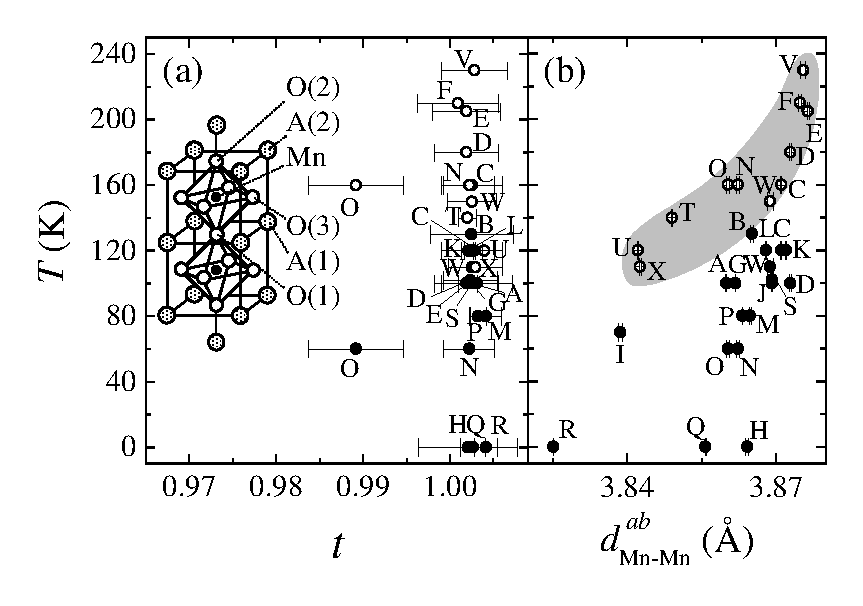
\includegraphics{fig1.eps}
 \caption{\label{fig1}Text of first caption.}
\end{figure}
\end{verbatim}
Note how the \cmd\label\marg{key} command is used to cross-reference
figures in text. The \cmd\label\marg{key} command should be inserted
inside the figure caption. As usual, the \cmd\ref\marg{key} macro can
then by used to refer to the label: ``As depicted in
FIG.\verb+~\ref{fig1}+\dots''.

Figures are normally set to the width of the column in
which they are placed. This means that in two-column mode, the figure
will be placed in a single, narrow column. For wide figures, the
\cmd\figure\verb+*+ environment should be used
instead. This will place the figure across both columns (the figure
usually will
appear either at the top or the bottom of the following page).


Captions less than one line long are centered under the figure,
otherwise they span the width of the figure.

Note that is unnecessary (and undesirable) to use explicit centering
commands inside the float environments.

\subsection{\texttt{video} environment}
Papers often refer to multimedia material such as videos. The \texttt{video} environment is identical to the \texttt{figure} environment, but the caption will be labeled as a \textbf{Video} (with its own counter independent of figures). A URL can also be specified so that the caption label can be linked to the online video (if using the \texttt{hyperref} package). The included graphic (using \cmd\includegraphics\ from the \texttt{graphics} or \texttt{graphicx} package) would be a representation frame from the video. A \texttt{\cmd\listofvideos} is also provided.  For example:
\begin{verbatim}
\begin{video}
\includegraphics{videoframe.jpg}
\setfloatlink{http://some.video.com/fun.mov}
\caption{\label{vid:interest}This is a video
of something fun.}
\end{video}
\end{verbatim}
There is also a corresponding \cmd\listofvideos\ command.

\section{Tables}\label{sec:tables}

Tables are very similar to figures. They should be input using the
\env{table} environment as detailed below, and 
\LaTeX\ will label and number the captions TABLE~1, TABLE~2, etc.
(or in whatever format required by the chosen journal
substyle). Tables without captions won't be numbered.

Each table must begin with \envb{table}, end with \enve{table}. A
caption can be specified using the \cmd\caption\marg{text} command.
Captions less than one line long are centered under the figure,
otherwise they span the width of the figure.
To refer to the table via cross-referencing, a \cmd\label\marg{key}
command should appear within the \cmd{\caption}.  Use the
\cmd\ref\marg{key} command to cite tables in text. The \env{table}
environment will set the table to the width of the column. Thus, in
two-column mode, the table will be confined to a single column. To set a
table to the full width of the page, rather than the column, use the
\env{table*} environment.

The heart of the table is the
\env{tabular} environment. This will behave for the most part as in
standard \LaTeXe\ (please refer to Section~3.6.3 and Appendix~C.10.2 of the
\LUG{} for more details about the \env{tabular} environment).
Note that \revtex~4.1 no longer automatically adds double (Scotch) rules
around tables. Nor does the \env{tabular} environment set various
table parameters for column spacing as before. Instead, a new
environment \env{ruledtabular} provides this functionality. This
environment should surround the \env{tabular} environment:
\begin{verbatim}
\begin{table}
\caption{\label{<key>}....}
\begin{ruledtabular}
\begin{tabular}
...
\end{tabular}
\end{ruledtabular}
\end{table}
\end{verbatim}

A basic table looks as follows:
\begin{verbatim}
\begin{table}
\caption{\label{tab:example}Text of table caption.}
\begin{ruledtabular}
\begin{tabular}{ll}
  Heading 1 & Heading 2\\
  Cell 1 & Cell 2\\
\end{tabular}
\end{ruledtabular}
\end{table}
\end{verbatim}

The \env{quasitable} environment is no longer in \revtex~4.1. The
standard \env{tabular} environment can be used instead because it
no longer puts in the double rules.

\subsection{Aligning on a decimal point}
Numerical columns should align on the decimal point (or
decimal points if more than one is is present). This is accomplished
by again using a standard \LaTeXe\ package, \classname{dcolumn} which
must be loaded in the manuscript's preamble:
\begin{verbatim}
\usepackage{dcolumn}
\end{verbatim}
Once this package is loaded, the column specifier `\texttt{d}' can be
used in the table's \env{tabular}\marg{preamble} enviroment preamble.
The `\texttt{d}' should be used for simple numeric data with a single
decimal point.
%
The entry of a \texttt{d} column is typeset in math mode; do not
insert any \verb+$+ math delimiters into a `\texttt{d}' column.  Items
without a decimal point are simply set in math mode, centered.  If
text is required in the column, use \cmd\text\ or \cmd\mbox\ as
appropriate.  If multiple decimal points are present then the last is
used for alignment. To escape from the `\texttt{d}' column use
\cmd\multicolumn\ as usual. See the sample file \file{apssamp.tex} for examples.

\subsection{Footnotes in Tables}\label{sec:tablenote}

Footnotes in a table are labeled \emph{a}, \emph{b}, \emph{c},
etc. They can be specified by using the \LaTeX\ \cmd\footnote\
command. Furthermore,
\cmd\footnotemark\ and \cmd\footnotetext\ can be used so that multiple entries
can to refer to the same footnote. The footnotes for a table are typeset
at the bottom of the table, rather than at the bottom of the page or
at the end of the references. The arguments for \cmd\footnotemark\ and
\cmd\footnotetext\ should be numbers 1, 2, \dots. The journal style
will convert these to letters.  See sample file \file{apssamp.tex} for
examples and explanations of use.

\subsection{Dealing with Long Tables}
By default, tables are set in a smaller size than the text body
(\cmd\small). The \cmd\squeezetable\ declaration makes the table font
smaller still (\cmd\scriptsize).  Thus, putting the
\cmd\squeezetable\ command before the \envb{table} line in a table
will reduce the font size. If this isn't sufficient to fit
the table on a page, the standard \LaTeXe\ \classname{longtable}
package may be used. The scope of the
\cmd\squeezetable\ command must be limited by enclosing it with a group:
\begin{verbatim}
\begingroup
\squeezetable
\begin{table}
[...]
\end{table}
\endgroup
\end{verbatim}

Tables are normally set to the width of the column in
which they are placed. This means that in two-column mode, the table
will be placed in a single, narrow column. For wide tables, the
\cmd\table\verb+*+ environment should be used
instead. This will place the table across both columns (the table
usually will
appear either at the top or the bottom of the following page).


To break tables across pages, \revtex~4.1requires adding to the
table a float placement option of [H] (meaning put the table ``here''
and effectively ``unfloating'' the table) to the \envb{table}
command. The commands \verb+\\*+ and \cmd{\samepage} can be used to
control where the page breaks occur (these are the same as for the
\env{eqnarray} environment).

Long tables are more robustly handled by using the
\classname{longtable.sty} package included with the standard \LaTeXe\
distribution (put \verb+\usepackage{longtable}+ in the preamble). This
package gives precise control over the layout of the table.
The \revtex~4.1 package contains patches that enable the
\classname{longtable} package to work in two-column mode. Of course, a
table set in two-column mode needs to be narrow enough to fit within
the column. Otherwise, the columns may overlap. \revtex~4.1 provides
an additional environment \env{longtable*} which allows a longtable to
span the whole page width. Currently, the \env{longtable*} and
\env{ruledtabular} environments are incompatible. In order to get the
double (Scotch) rule, it is necessary to add the \verb+\hline\hline+
manually (or define \verb+\endfirsthead+ and \verb+\endlastfoot+
appropriately).  For more documentation on the \env{longtable}
environment and on the package options of the
\classname{longtable} package, please see the documentation available at
\url{http://www.ctan.org/macros/latex/required/tools/longtable.dtx} or
refer to \cite{Compan}.

\section{Placement of Figures, Tables, and Other Floats}
\label{sec:place}

By default, figures and tables (and any other ``floating'' environments
defined by other packages) float to the top or bottom of the page
using the standard \LaTeX\ float placement mechanism.  Initially, each
\env{figure} or \env{table} environment should be put immediately
following its first reference in the text; this will usually result in
satisfactory placement on the page.  An optional argument for either 
environment adjusts the float placement. For example:
\begin{quote}
\envb{figure}\oarg{placement}\\
\dots\\
\enve{figure}
\end{quote}
where \meta{placement} can be any combination of \verb|htbp!|, signifying
``here'', ``top'', ``bottom'', ``page'', and ``as soon as possible'',
respectively. The same placement argument may be added to a
\envb{table}. For more details about float placement, 
see the instructions in the \LUG, Appendix~C.9.1.

In two-column mode, a page may contain both a \env{widetext}
environment and a float. \revtex~4.1 may not always be able to
automatically put the float in the optimal place. For instance, a
float may be placed at the bottom of a column just before the
\env{widetext} begins. To workaround this, try moving the float
environment below the \env{widetext} environment. Alternative
\meta{placements} may also alleviate the problem.

\env{figure} and \env{table} environments should not 
be enclosed in a \env{widetext} environment to make them span
the page to accommodate wide figures or tables. Rather, the
\env{figure*} or \env{table*} environments should be used instead.

Sometimes in \LaTeX\ the float placement mechanism breaks down and a
float can't be placed. Such a ``stuck'' float may mean that it and all
floats that follow are moved to the end of the job (and if there are
too many of floats, the fatal error \texttt{Too many unprocessed floats}
will occur). \revtex~4.1 provides the class option
\classoption{floatfix} which attempts to invoke emergency float
processing to avoid creating a ``stuck'' float. \revtex~4.1 will provide
a message suggesting the use of
\classoption{floatfix}. If \classoption{floatfix} doesn't work or if
the resulting positioning of the float is poor, the float should be
repositioned by hand.

\revtex~4.1 offers an additional possibility for placing the floats. By
using the either the \classoption{endfloats} or the
\classoption{endfloats*} class option all floats may be held
back (using an external file) and then set elsewhere in the document
using the the commands \cmd\printtables\ and \cmd\printfigures{},
placed where the tables and figures are to be printed (usually at the
end of the document).  (This is similar to the standard
\cmd\printindex\ command). Using a \texttt{*}-form of the commands
(\cmd\printfigures\verb+*+ and
\cmd\printtables\verb+*+) will begin the figures
or tables on a new page. Alternatively, the option
\classoption{endfloats*} may be used to change the behavior of the
non-\texttt{*}-forms so that every float will appear on a separate
page at the end.

Without one of the \classoption{endfloats} class options, these float
placement commands are silently ignored, so it is always safe to use
them.  If one of the \classoption{endfloats} class options is given,
but the \cmd\printtables\ command is missing, the tables will be
printed at the end of the document. Likewise, if \cmd\printfigures\ is
missing, the figures will be printed at the end of the document.
Therefore it is also safe to omit these commands as long as \revtex's
default choices for ordering figures and tables are satisfactory.

The \classoption{endfloats} option (or perhaps some journal substyle
that invokes it), requires explicit \envb{figure}, \enve{figure},
\envb{table}, and \enve{table} lines. In particular, do \emph{not}
define typing shortcuts for table and figure environments, such as
\begin{verbatim}
\def\bt{\begin{table}}% Incompatible!
\def\et{\end{table}}%
\end{verbatim}

Please note that it is generally undesirable to have all floats moved
to the end of the manuscript. APS no longer requires this for
submissions. In fact, the editors and referees will have an easier time
reading the paper if the floats are set in their normal positions.

\section{Rotating Floats}

Often a figure or table is too wide to be typeset in the standard
orientation and it is necessary to rotate the float 90
degrees. \revtex~4.1 provides a new environment \env{turnpage} as an
easy means to accomplish this. The \env{turnpage} environment depends
on one of the packages \classname{graphics} or \classname{graphicx}
being loaded. To use the \env{turnpage} environment, simply enclose
the \env{figure} or \env{table} environment with the \env{turnpage}
environment:
\begin{verbatim}
\documentclass[...]{revtex4}
\usepackage{graphicx}
[...]
\begin{turnpage}
\begin{figure} or \begin{table}
[...]
\end{figure} or \end{table}
\end{turnpage}
\end{verbatim}
A turnpage float will be typeset on a page by itself. Currently, there
is no mechanism for breaking such a float across multiple pages.

\section{\revtex~4.1 symbols and the \classname{revsymb4-1} package}

Symbols made available in earlier versions of \revtex\ are
defined in a separate package, \classname{revsymb4-1},
so that they may be used with other classes.
This might be useful if, say, copying text from a \revtex\ document to
a non-\revtex\ document. \revtex~4.1 automatically includes these
symbols so it is not necessary to explicitly call them in with a 
\cmd\usepackage\ statement.

Table~\ref{tab:revsymb} summarizes the symbols defined in this package.
Note that \cmd{\overcirc}, \cmd{\overdots}, and \cmd{\corresponds} are
no longer in \revtex~4.1. Use \cmd{\mathring} (standard in \LaTeXe),
\cmd{\dddot} (with the \classoption{amsmath} package loaded), and 
\cmd\triangleq\ (with the \classoption{amssymb} class option) respectively.
\cmd{\succsim}, \cmd{\precsim}, \cmd{\lesssim}, and \cmd{\gtrsim} are
also defined either in \classname{amsmath} or \classname{amssymb}. The
AMS versions of these commands will be used if the appropriate AMS
package is loaded.

\begin{table}
\caption{\label{tab:revsymb}Special \revtex~4.1 symbols, accents, and
boldfaced parentheses defined in \file{revsymb.sty}}
\begin{ruledtabular}
\begin{tabular}{ll|ll}
\cmd\lambdabar & $\lambdabar$ &\cmd\openone & $\openone$\\
\cmd\altsuccsim & $\altsuccsim$ & \cmd\altprecsim & $\altprecsim$ \\
\cmd\alt & $\alt$ & \cmd\agt & $\agt$ \\
\cmd\tensor\ x & $\tensor x$ & \cmd\overstar\ x & $\overstar x$ \\
\cmd\loarrow\ x & $\loarrow x$ & \cmd\roarrow\ x & $\roarrow x$  \\
\cmd\biglb\ ( \cmd\bigrb ) & $\biglb( \bigrb)$ &
\cmd\Biglb\ ( \cmd\Bigrb )& $\Biglb( \Bigrb)$ \\
& & \\
\cmd\bigglb\ ( \cmd\biggrb ) & $\bigglb( \biggrb)$ &
\cmd\Bigglb\ ( \cmd\Biggrb\ ) & $\Bigglb( \Biggrb)$ \\
\end{tabular}
\end{ruledtabular}
\end{table}

\section{Other \revtex~4.1 Features}
%\subsection{Hooks}
%To be written....

\subsection{Job-specific Override Files}
\revtex~4.1 allows manuscript-specific macro definitions to be put
in a file separate from the main \TeX\ file. One merely creates a file
with the same basename as the \TeX\ file, but with the extension
`.rty'. Thus, if the \TeX\ file is names man.tex, the macro
definitions would go in man.rty. Note that the .rty file should be in
the same directory as the \TeX\ file. APS authors should follow the
guidelines in the \textit{APS Author Guide for \revtex~4.1} when
submitting. Similarly, AIP authors should refer to the \textit{Author's Guide to AIP Substyles for \revtex~4.1}


\begin{thebibliography}{}\label{sec:TeXbooks}
\bibitem[Knuth(1986)]{TeXbook} D.E. Knuth, \emph{The \TeX book},
(Addison-Wesley, Reading, MA, 1986).
\bibitem[Lamport(1996)]{LaTeXman} L. Lamport, \emph{\LaTeX, a Document
Preparation System}, (Addison-Wesley, Reading, MA, 1996).
\bibitem[Kopka(1995)]{Guide} H. Kopka and P. Daly, \emph{A Guide to
\LaTeXe}, (Addison-Wesley, Reading, MA, 1995).
\bibitem[Goossens(1994)]{Compan} M. Goossens, F. Mittelbach, and
A. Samarin, \emph{The \LaTeX\
Companion}, (Addison-Wesley, Reading, MA, 1994).
\bibitem[Goossens(1997)]{CompanG} M. Goossens, S. Rahtz, and
F. Mittelbach, \emph{The
\LaTeX\ Graphics Companion}, (Addison-Wesley, Reading, MA, 1997).
\bibitem[Rahtz(1999)]{CompanW} S. Rahtz, M. Goossens, \emph{et
al.},\emph{The \LaTeX\ Web Companion}, (Addison-Wesley, Reading, MA, 1999).
\end{thebibliography}

\end{document}

